\documentclass[a4paper]{article}

% Options possibles : 10pt, 11pt, 12pt (taille de la fonte)
%                     oneside, twoside (recto simple, recto-verso)
%                     draft, final (stade de développement)
\usepackage{graphicx}
\usepackage[utf8]{inputenc}
\usepackage[T1]{fontenc}
\usepackage[francais]{babel} 

\usepackage[a4paper]{geometry}

\title{Calcul de couture minimale}         
\author{Maxime Broy \and Florent Guiotte}
\date{}                   

\sloppy
\begin{document}
\maketitle {ESIR3 - Imagerie Numérique - CAV - Projet}
\begin{abstract}
L'objectif initial du projet était l'implémentation du papier Scene Completion Using Millions of Photographs [Hays et Efros. 2007]. Ce dernier consiste à remplacer dans une image toute une région par une scène présente dans une autre image provenant d'une collection de photographies. L'algorithme explore cette collection jusqu'à trouver une image avec une sémantique correspondante. On cherche donc à remplacer une région de l'image cible par quelque chose de "plausible". Il s'agit d'une technique difficilement quantifiable puisque le résultat repose sur la perception visuel humaine. En pratique, ce projet s'est concentré sur une des briques de cette algorithme : le calcul de la couture minimale entourant l'objet que l'on veut transférer d'une image à une autre. 
\end{abstract}

% \tableofcontents              % Table des matières



\section{Introduction et concept}               % Commencer une section, etc.

\begin{figure}[!h]
	\begin{minipage}[b]{0.40\linewidth}
    	\centering 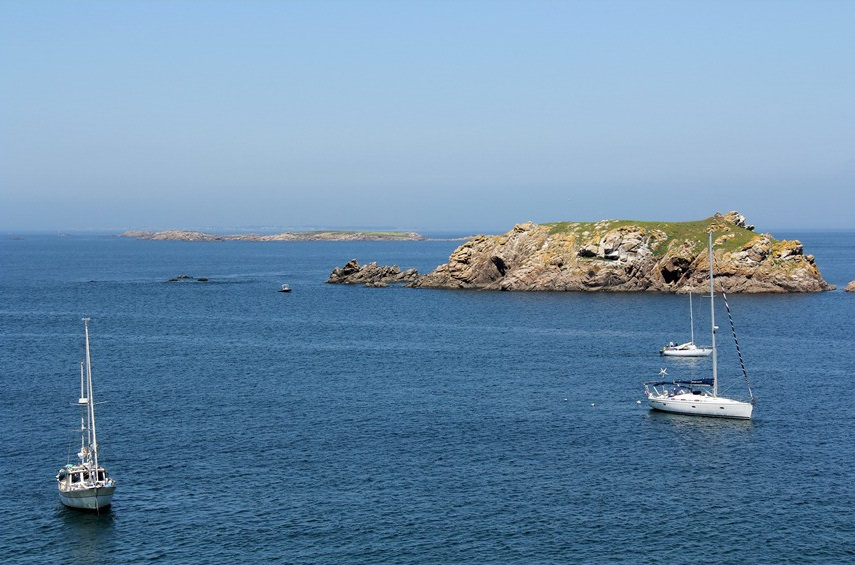
\includegraphics[width=6.5cm, height=5cm]{bg.jpg}
    	\caption{\it image cible}
    \end{minipage}\hfill
    \begin{minipage}[b]{0.40\linewidth}
    	\centering 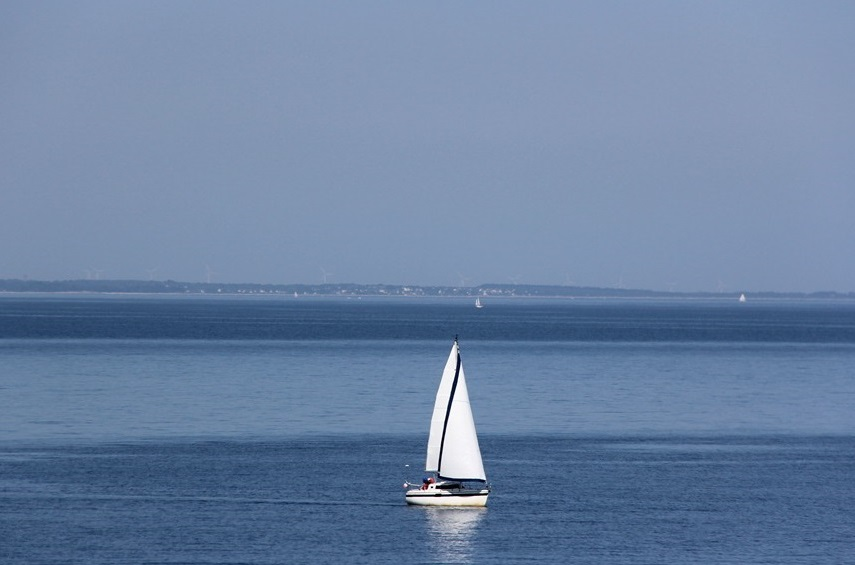
\includegraphics[width=6.5cm, height=5cm]{fg.jpg}
    	\caption{\it image source}
    \end{minipage}\hfill
\end{figure}

L'idée est de "découper" une région dans l'image source, ici la biche de la Figure 2 pour la transposer dans l'image cible. La biche devra alors s'intégrer le plus parfaitement possible dans son environnement. L'idée est donc de calculer quels sont les pixels entourant la biche que nous allons transposer avec elle dans l'image cible.

\section{Méthode}         
Notre méthode consiste à obtenir un masque de l'image source (Figure 2) en utilisant la fonction GrabCut d'OpenCV. Ensuite, nous calculons l'énergie entre les deux images. C'est en utilisant le masque en sortie du GrabCut et l'énergie que nous pouvons ensuite calculer les cartes d'énergie cumulée. La couture qui minimise cette énergie cumulée sera celle retenue.

\subsection{Grabcut}      
On utilise la fonction GrabCut d'Open CV.
\begin{figure}[!h]
	\begin{minipage}[b]{0.40\linewidth}
    	\centering 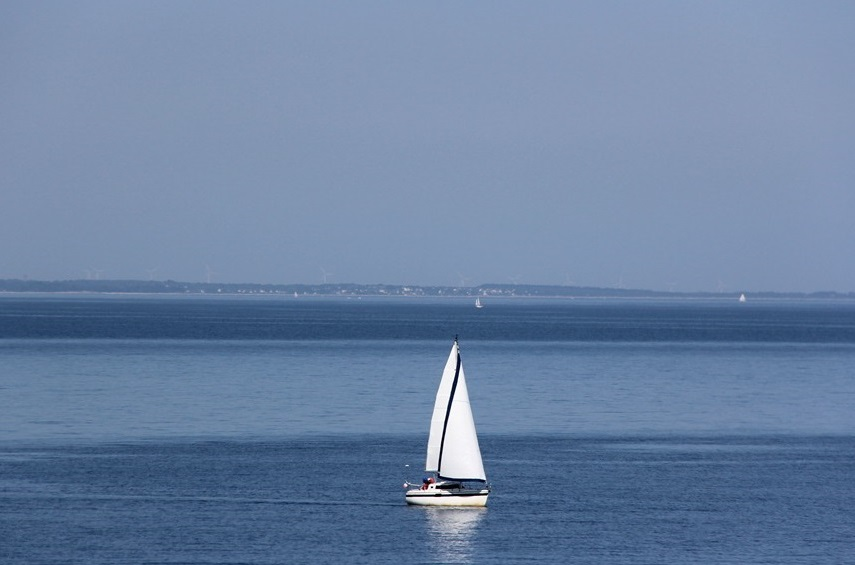
\includegraphics[width=6.5cm, height=5cm]{fg.jpg}
    	\caption{\it image source}
    \end{minipage}\hfill
    \begin{minipage}[b]{0.40\linewidth}
    	\centering 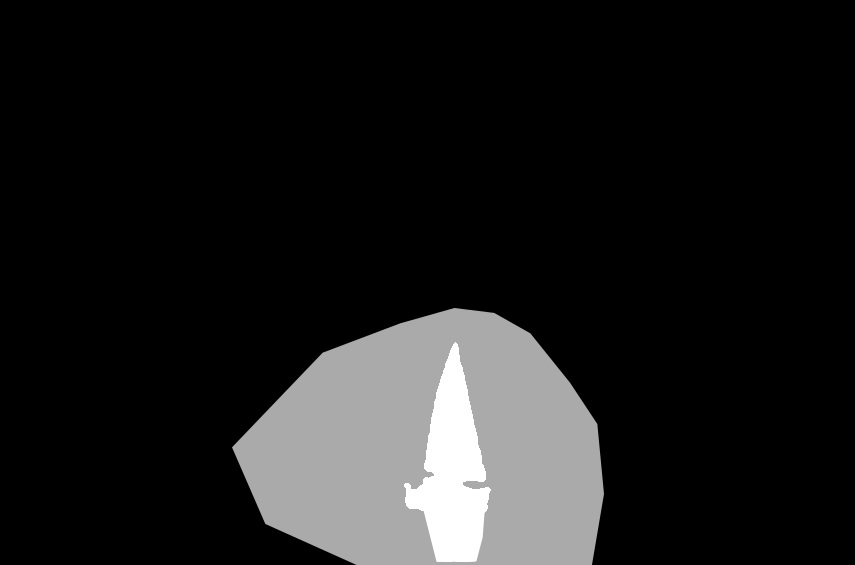
\includegraphics[width=6.5cm, height=5cm]{mask.png}
    	\caption{\it masque}
    \end{minipage}\hfill
\end{figure}

L'algorithme du grabcut permet d'extraire le fond d'une image. 
Le masque obtenu en Figure 4 contient trois valeurs différentes : 0 (noir), 170 (gris), 255 (blanc) Le gris correspond à une zone ayant une forte probabilité d'appartenir au fond. C'est dans cette zone que nous allons chercher la couture minimale.

\subsection{Calcul d'énergie}

Nous avons essayé plusieurs techniques pour ce calcul d'énergie : Différence au carrée entre les deux images, Sobel en RBG ou LAB.
Voici le résultat pour une énergie calculée à partir de la différence au carrée :
\begin{figure}[!h]
	\begin{minipage}[b]{0.40\linewidth}
    	\centering 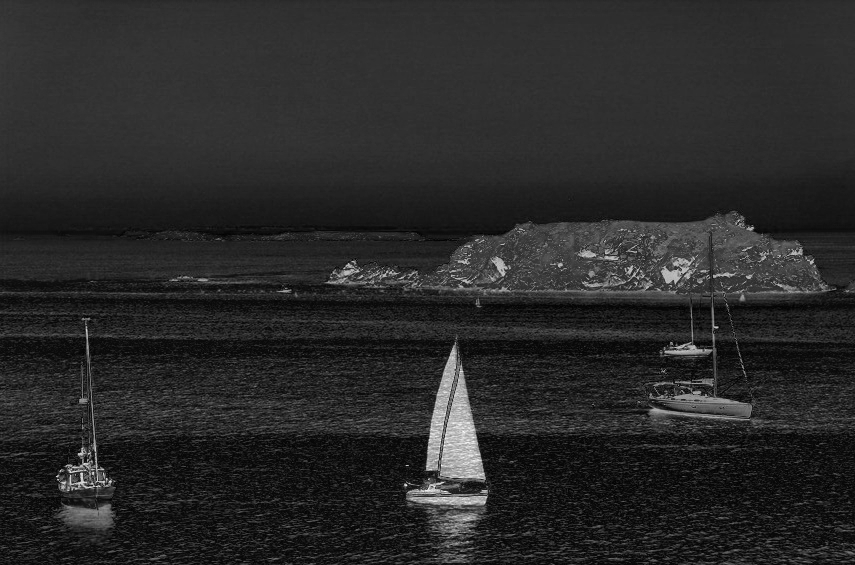
\includegraphics[width=6.5cm, height=5cm]{energy.png}
    	\caption{\it Energie : valeur absolue de la différence au carrée}
    \end{minipage}\hfill\begin{minipage}[b]{0.40\linewidth}
    	\centering 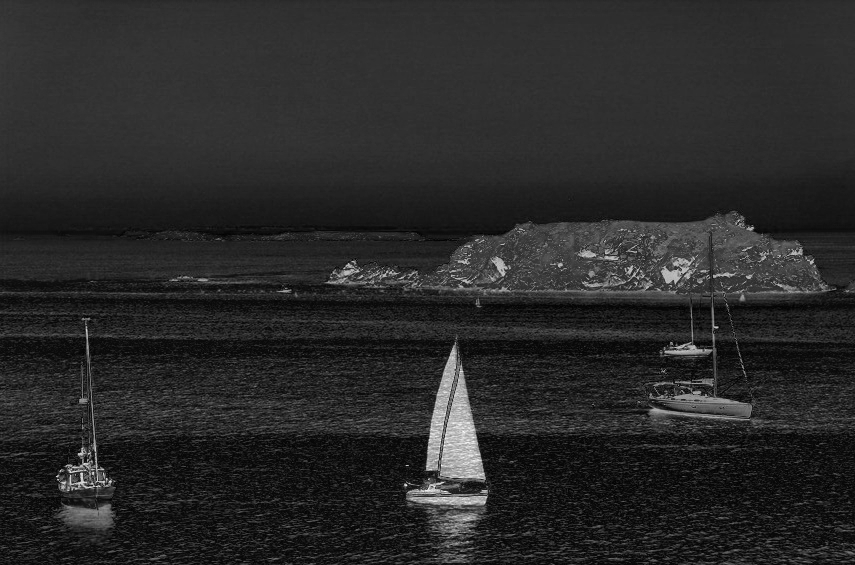
\includegraphics[width=6.5cm, height=5cm]{energy.png}
    	\caption{\it Energie : Sobel}
    \end{minipage}\hfill
\end{figure}


\subsection{Calcul des cartes d'énergie cumulée}
\begin{figure}[!h]
	\begin{minipage}[b]{0.40\linewidth}
    	\centering \includegraphics[width=6.5cm, height=5cm]{steam.png}
    	\caption{\it Masque avec la ligne de départ}
    \end{minipage}\hfill
    \begin{minipage}[b]{0.40\linewidth}
    	\centering \includegraphics[width=6.5cm, height=5cm]{energie_cumulee.png}
    	\caption{\it énergie cumulée}
    \end{minipage}\hfill
\end{figure}

Tout d'abord, il faut définir une ligne de pixels partant du bord du masque jusqu'à l’objet (on appellera cette ligne steam, pour start seam). Il s'agit de la ligne rouge sur la Figure 6.
Il y a une carte d’énergie par pixels de la steam.
Une carte d’énergie correspond à l’énergie cumulée de chaque pixel, en partant d’un pixel de steam jusqu’à faire le tour de l’objet en explorant le voisinage (connexité 8)

\subsection{Calcul de la couture}

\begin{figure}[!h]
    	\centering \includegraphics[width=11.5cm, height=8cm]{minseam_best.png}
    	\caption{\it Couture minimale}
\end{figure}
Pour chaque pixel qui n’est pas noir et qui n’est pas déjà visité, on explore ses voisins en sélectionnant celui dont l’énergie correspondante (dans la carte d’énergie) est minimale. Cela jusqu'à avoir atteint le point d'arrivée (voisin de droite du point de départ).

\section{Résultat}

Quisque dolor odio, aliquam quis, placerat sed, hendrerit eu, magna. Cras at
turpis et mi imperdiet lobortis. Nam eu massa et eros congue gravida. Sed
luctus. Nullam sit amet nunc a tellus lacinia tempor. Praesent tincidunt ligula
quis lacus. Nullam sodales, mi sed venenatis egestas, risus turpis dictum elit,
ac egestas augue eros eget erat. Cras faucibus.

\section{Performance}

Quisque dolor odio, aliquam quis, placerat sed, hendrerit eu, magna. Cras at
turpis et mi imperdiet lobortis. Nam eu massa et eros congue gravida. Sed
luctus. Nullam sit amet nunc a tellus lacinia tempor. Praesent tincidunt ligula
quis lacus. Nullam sodales, mi sed venenatis egestas, risus turpis dictum elit,
ac egestas augue eros eget erat. Cras faucibus.

\section{Références}

[1] J. Hays and A. A. Efros.  2007. Scene completion using millions of photographs. ACM Trans. Graph.,
\\

[2] JIA, J., SUN, J., TANG, C.-K., AND SHUM, H.-Y. 2006. Drag and-drop pasting. ACM Trans. Graph.,



\end{document}
